\chapter{Решение задачи анализа потокового графа с использованием методики GERT и алгебры потоковых графов}
\section{Постановка задачи}
\textbf{Вариант:} 36.\\\\
\textbf{Дано:}
\begin{enumerate}
\item Граф GERT-сети
\begin{figure}[H]
  \centering
  \fbox{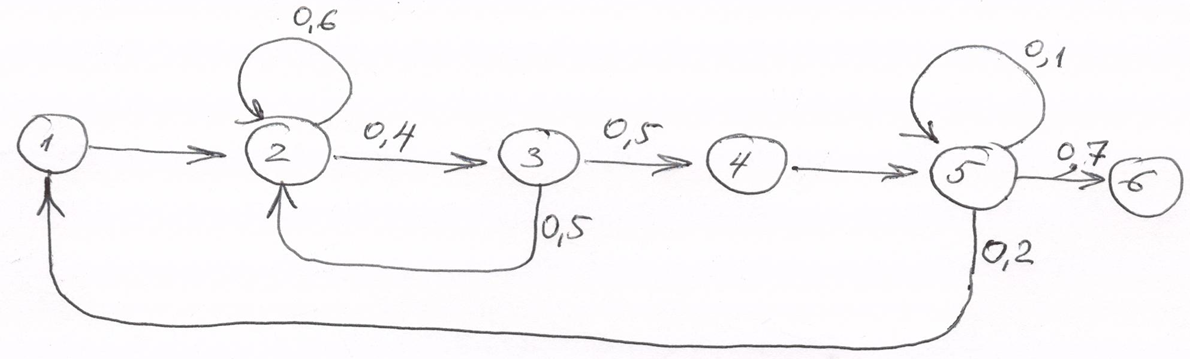
\includegraphics[width=.85\textwidth]{img/scheme_0}}
  \caption{Граф GERT-сети}
\end{figure}
\item Каждой дуге-работе ($ij$) поставлены в соответствие следующие данные:
\begin{enumerate}
\item Закон распределения времени выполнения работы. Будем считать его нормальным;
\item Параметры закона распределения (математическое ожидание \textbf{M} и дисперсия \textbf{D});
\item Вероятность $p_{ij}$ выполнения работы, показанная на графе.
\end{enumerate}
\end{enumerate}


\subsection{Задание}
\subsubsection{Часть 1}
Используя методику GERT, изложенную в книге «Методы анализа сетей»\\
Найти:
\begin{enumerate}
\item Вероятность выхода в завершающий узел графа (для всех вариантов узел 6);
\item Производящую функцию длительности процесса от начального узла  до завершающего узла;
\item Математическое ожидание длительности процесса от начального узла  до завершающего узла;
\item Дисперсию ожидание длительности процесса от начального узла  до завершающего узла;
\end{enumerate}
В отчете перечислить все петли всех порядков, обнаруженные на графе, выписать уравнение Мейсона, получить решение для $W_E(S)$ и найти требуемые параметры. Примерно так, как это сделано в примере на стр. 403–409 книги Филипса и Гарсиа «Методы анализа сетей»
\subsubsection{Часть 2}
Повторить пункты задания 2, 3, 4 используя методику анализа потокового графа, основанную на обработке матрицы передач (Branch Transmittance Matrix). 


Для выполнения задания рекомендуется пользоваться следующими источниками:
\begin{enumerate}
\item Филипс и Гарсиа «Методы анализа сетей»
\item Презентация GERT\_\&\_Flowgraph\_Algebra.pdf (выложена в ИНТРАНЕТ)
\item Ren\_The Methodology of Flowgraph.pdf
\end{enumerate}

\section{Решение}

\subsection{Часть 1}
Чтобы определить эквивалентную W-функцию для анализируемой GERT-сети, необходимо замкнуть сеть дугой, исходящей из узла 6 в узел 1 (рис. \ref{pic_1}).
\begin{figure}[H]
  \centering
  \fbox{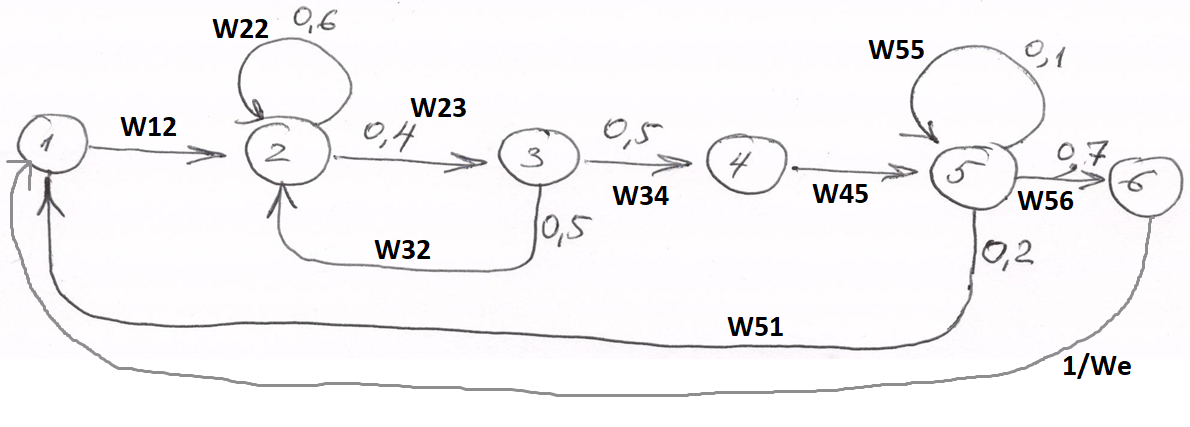
\includegraphics[width=\textwidth]{img/scheme_1}}
  \caption{Замкнутая GERT-сеть}
  \label{pic_1}
\end{figure}
Далее, выпишем в таблицу данные графа(мат. ожидание, дисперсия, W-функции)

\tabulinesep = 1mm
\begin{longtabu} to \textwidth {|X[8,c , m ] |X[8,c , m ] | X[15,l, m ]| X[15,l, m ]|X[15,l, m ]|X[25,l, m ]|}\firsthline\hline
\textbf{Начало}&\textbf{Конец}&\textbf{Вес ребра}&\textbf{Мат. ожидание}&\textbf{Дисперсия}&\textbf{W-функция}\\ \hline \endfirsthead
1	&2	&1	&20	&9	&$exp(20s+4.5s^2)$	\\ \hline
2	&2	&0.6&30	&16	&$0.6*exp(30s+8s^2)$	\\ \hline
2	&3	&0.4&40	&25	&$0.4*exp(40s+12.5s^2)$	\\ \hline
3	&2	&0.5&28	&16	&$0.5*exp(28s+8s^2)$	\\ \hline
3	&4	&0.5&37	&16	&$0.5*exp(37s+8s^2)$	\\ \hline
4	&5	&1	&30	&25	&$exp(30s+12.5s^2)$	\\ \hline
5	&1	&0.2&30	&16	&$0.2*exp(30s+8s^2)$	\\ \hline
5	&5	&0.1&10	&4	&$0.1*exp(10s+2s^2)$	\\ \hline
5	&6	&0.7&30	&16	&$0.7*exp(30s+8s^2)$	\\ \hline
\caption{Данные анализируемой GERT-сети}
\end{longtabu}
\textbf{Петли первого порядка:}
\begin{itemize}
\item $W_{12}W_{23}W_{34}W_{45}W_{51}$;
\item $W_{12}W_{23}W_{34}W_{45}W_{56}\frac{1}{W_e}$;
\item $W_{22}$;
\item $W_{23}W_{32}$;
\item $W_{55}$;
\end{itemize}
\textbf{Петли второго порядка:}
\begin{itemize}
\item $W_{22}W_{55}$;
\item $W_{55}W_{23}W_{32}$;
\end{itemize}
\textbf{Уравнение Мейсона}:
\begin{multline*}
H = 1 - W_{12}W_{23}W_{34}W_{45}W_{51} - W_{12}W_{23}W_{34}W_{45}W_{56}\frac{1}{W_e} - W_{22} - W_{23}W_{32} - W_{55}\\
 + W_{22}W_{55} + W_{55}W_{23}W_{32} = 0
\end{multline*}
\textbf{Выведем $W_E(S)$:}
\begin{equation*}
1 - W_{12}W_{23}W_{34}W_{45}W_{51} - W_{22} - W_{23}W_{32} - W_{55} + W_{22}W_{55} + W_{55}W_{23}W_{32} = W_{12}W_{23}W_{34}W_{45}W_{56}\frac{1}{W_e}
\end{equation*}
\begin{multline*}
W_E(S) =\\
(W_{12}W_{23}W_{34}W_{45}W_{56})/(1 - W_{12}W_{23}W_{34}W_{45}W_{51} - W_{22} - W_{23}W_{32} - W_{55} + W_{22}W_{55} + W_{55}W_{23}W_{32})
\end{multline*}

Вычислим математическое ожидание и дисперсию: $M_E(s) = 1$ при $s=0$

Так как $W_E(s)=p_E M_E (s)$,  то  $p_E=W_E(0)$, тогда $M_E(s)=\frac{W_E(s)}{p_E} =\frac{W_E(s)}{W_E(0)}$

Вычисляя первую и вторую производные по $s$ функции $M_E(s)$, и полагая $s=0$, находим математическое ожидание:
\begin{equation*}
\mu_{1E}=\frac{\partial M_E(s)}{\partial s}|s=0
\end{equation*}

и дисперсию:
\begin{equation*}
\sigma^2=\mu_{2E}-[\mu_{1E}]^2
\end{equation*}

Вероятность выхода в завершающий узел графа:
\begin{equation*}
p_E=W_E (0)
\end{equation*}
Для решения задачи был написан скрипт matlab, код приведен в приложении 4.

\begin{lstlisting}[language={matlab}, caption={Результат}, basicstyle=\ttfamily]
We =
-(7*exp((s*(91*s + 314))/2))/(5*exp(2*s*(s + 5)) - 3*exp(10*s*(s + 4)) + 30*exp(2*s*(4*s + 15)) - exp((3*s*(15*s + 52))/2) + 10*exp((s*(41*s + 136))/2) + 2*exp((s*(91*s + 314))/2) - 50)
 
We0 =
1
 
m1 =
2845/7
 
m2 =
11938987/49
 
D =
3844962/49
\end{lstlisting}
Были получены следующие результаты:
\begin{enumerate}
\item Вероятность выхода в завершающий узел графа равна 100\% ($p=W_E=1$).
\item Математическое ожидание 406,43.
\item Дисперсия времени выхода процесса в завершающий узел графа 78 468,61.
\end{enumerate}
\subsection{Часть 2}
Алгоритм дальнейших действий основан на:
\begin{itemize}
\item Презентация GERT\_\&\_Flowgraph\_Algebra.pdf (со слайда 56);
\item Ren\_The Methodology of Flowgraph.pdf (со страницы 35).
\end{itemize}
Определим матрицу Q, не забывая про обратную связь.
\begin{equation*}
Q = 
 \begin{pmatrix}
  0 & q_{12} & 0 & 0 & 0 & 0 \\
  0 & q_{22} & q_{23} & 0 & 0 & 0 \\ 
  0 & q_{32} & 0 & q_{34} & 0 & 0 \\ 
  0 & 0 & 0 & 0 & q_{45} & 0 \\ 
  q_{51} & 0 & 0 & 0 & q_{55} & q_{56} \\ 
  w_{61} & 0 & 0 & 0 & 0 & 0 
 \end{pmatrix}
\end{equation*}
Определим матрицу коэффициентов $A=I_6-Q^T$.
\begin{equation*}
A = 
 \begin{pmatrix}
    1&       0&    0&    0&    -q_{51}& -w_{61}\\
 -q_{12}& 1 - q_{22}& -q_{32}&    0&       0&    0\\
    0&    -q_{23}&    1&    0&       0&    0\\
    0&       0& -q_{34}&    1&       0&    0\\
    0&       0&    0& -q_{45}& 1 - q_{55}&    0\\
    0&       0&    0&    0&    -q_{56}&    1
 \end{pmatrix}
\end{equation*}
Находим 
\begin{equation*}
det(A)
\end{equation*}
далее
\begin{equation*}
\frac{\partial det(A)}{\partial w_{61}}
\end{equation*}
\begin{equation*}
det(A | w_{61}=0)
\end{equation*}
Далее можно вывести $W_E(S)$ с помощью формулы:
\begin{equation*}
W_E(S)=-\frac{\frac{\partial det(A)}{\partial w_{61}}}{det(A | w_{61}=0)}
\end{equation*}
Для расчетов, был написан matlab скрипт, код представлен в приложении 5.

\begin{lstlisting}[language={matlab}, caption={Результат}, basicstyle=\ttfamily]
[    1,       0,    0,    0,    -q51, -w61]
[ -q12, 1 - q22, -q32,    0,       0,    0]
[    0,    -q23,    1,    0,       0,    0]
[    0,       0, -q34,    1,       0,    0]
[    0,       0,    0, -q45, 1 - q55,    0]
[    0,       0,    0,    0,    -q56,    1]
 
 
-(q12*q23*q34*q45*q56)/(q22 + q55 + q23*q32 - q22*q55 - q23*q32*q55 + q12*q23*q34*q45*q51 - 1)
\end{lstlisting}
Во второй строчке был получен $W_E(S)$, который полностью(за исключением знаков) совпадает с $W_E(S)$ найденным в части 1.

Далее, имея $W_E(S)$ находим необходимые переменные.

Для расчетов, был использован скрипт из приложения 6.

\begin{lstlisting}[language={matlab}, caption={Результат}, basicstyle=\ttfamily]
We =
-(7*exp((s*(91*s + 314))/2))/(5*exp(2*s*(s + 5)) - 3*exp(10*s*(s + 4)) + 30*exp(2*s*(4*s + 15)) - exp((3*s*(15*s + 52))/2) + 10*exp((s*(41*s + 136))/2) + 2*exp((s*(91*s + 314))/2) - 50)
 
We0 =
1
 
m1 =
2845/7
 
m2 =
11938987/49
 
D =
3844962/49
\end{lstlisting}
Были получены следующие результаты:
\begin{enumerate}
\item Вероятность выхода в завершающий узел графа равна 100\% ($p=W_E=1$).
\item Математическое ожидание 406,43.
\item Дисперсия времени выхода процесса в завершающий узел графа 78 468,61.
\end{enumerate}
Которые полностью совпадает с результатами части 1.